\newpage
\section{2023秋}

\setcounter{yearcounter}{2023}
% \setcounter{page}{1}

\subsection{微分積分}
\prob{%
  次のように\dm{x,y}が変数\dm{t}の関数として与えられるとき、
  \dm{x,y}を用いて\dm{\frac{dy}{dx}}を表せ。
  \begin{align}
    \begin{dcases*}
      x = \frac{2t}{t^2 + 1} \\
      y = \frac{t^2 - 1}{t^2 + 1} \\
    \end{dcases*}
  \end{align}
}
\begin{ans*}
  与式より$x^2 + y^2 = 1$であるので両辺を$x$で微分して
  \begin{gather}
    2x + 2y\frac{dy}{dx} = 0 \\
    \frac{dy}{dx} =
    \begin{dcases*}
      0 & if $y=0$ \\
      -\frac{x}{y} & o/w
    \end{dcases*}
  \end{gather}

\end{ans*}
\prob{%
  以下の問いに答えよ。
  \begin{enumerate}[label=(\arabic*)]
    \item 次に示す関数\dm{f(t)}および\dm{g(t)}を\dm{t=0}のまわりでそれぞれテイラー展開せよ。
    \begin{align}
      f(t) = \sin t,\quad g(t) = \cos t
    \end{align}
    \item 次に示す2次の正方行列\dm{\bA}と単位行列\dm{\bE}を考える。
    \dm{n}をゼロ以上の整数とし、\dm{n,t,\bE}を用いて\dm{\bA^2}および
    \dm{\bA^{2n}}を表せ。なお、\dm{\bA^0}は\dm{\bE}と定義される。
    \begin{align}
      \bA =
      \pmat{
        0 & -t \\
        t & 0
      }
      ,\quad
      \bE =
      \pmat{
        1 & 0 \\
        0 & 1
      }
    \end{align}
    \item 行列\dm{\bA}の指数関数\dm{\exp \bA}は次のように定義される。
    \dm{\sin t}と\dm{\cos t}を用いて\dm{\exp \bA}のすべての成分を表せ。
    \begin{align}
      \exp\bA = \sum_{k=0}^{\infty}\frac{1}{k!}\bA^k = \bE + \frac{1}{1!}\bA + \frac{1}{2!}\bA^2 + \cdots
    \end{align}
  \end{enumerate}
}
\begin{ans*}
  ${}$
  \begin{enumerate}[label=(\arabic*)]
    \item $t=0$まわりのテイラー展開はそれぞれ
    \begin{align}
      f(t)
      &= \sum_{n=0}^{\infty} \frac{f^{(n)}(0)}{n!} t^n \\
      &= t - \frac{t^3}{3!} + \frac{t^5}{5!} - \frac{t^7}{7!} + \cdots \\
      g(t)
      &= 1 - \frac{t^2}{2!} + \frac{t^4}{4!} - \frac{t^6}{6!} + \cdots
    \end{align}
    \item 与えられた行列について、$\bA^2$は
    \begin{align}
      \bA^2
      &=
      \bmat{
        0 & -t \\
        t & 0
      }
      \bmat{
        0 & -t \\
        t & 0
      } \\
      &= -t^2
      \bmat{
        1 & 0 \\
        0 & 1
      } \\
      &= -t^2 \bE
    \end{align}
    また、$\bA^{2n}$は
    \begin{align}
      \bA^{2n}
      &=
      \begin{dcases*}
        (-t^{2})^{n}\bE & if $n\geq 1$ \\
        \bE & if $n = 0$
      \end{dcases*} \\
      &= (-t^{2})^{n}\bE
    \end{align}
    \item (2)より
    \begin{align}
      \exp\bA
      &=
      \bE + \frac{1}{2!}\bA^2 + \frac{1}{4!}\bA^4 + \frac{1}{6!}\bA^6 + \cdots
      + \frac{1}{1!}\bA + \frac{1}{3!}\bA^3 + \frac{1}{5!}\bA^5 + \cdots \\
      &=
      \bE - \frac{t^2}{2!}\bE + \frac{t^4}{4!}\bE - \frac{t^6}{6!}\bE + \cdots
      + \frac{1}{1!}\bA - \frac{t^2}{3!}\bA + \frac{t^4}{5!}\bA - \cdots \\
      &=
      \bE - \frac{t^2}{2!}\bE + \frac{t^4}{4!}\bE - \frac{t^6}{6!}\bE + \cdots
      + \frac{1}{1!}\bA - \frac{t^2}{3!}\bA + \frac{t^4}{5!}\bA - \cdots \\
      &=
      \biggl(1 - \frac{t^2}{2!} + \frac{t^4}{4!} - \frac{t^6}{6!} + \cdots \biggr)\bE
      + \biggl(\frac{t}{1!} - \frac{t^3}{3!} + \frac{t^5}{5!} - \cdots \biggr)
      \pmat{
        0 & -1 \\
        1 & 0
      } \\
      &=
      \cos t
      \pmat{
        1 & 0 \\
        0 & 1
      }
      +
      \sin t
      \pmat{
        0 & -1 \\
        1 & 0
      } \\
      &=
      \pmat{
        \cos t & -\sin t \\
        \sin t & \cos t
      }
    \end{align}

  \end{enumerate}

\end{ans*}

\prob{%
  次の重積分について、以下の問いに答えよ。
  \begin{align}
    I = \iint_D x \,dx dy,\quad D = \left\{(x,y)\relmiddle x\geq 0, y\geq 0, 1\leq x^2 + y^2\leq 2y\right\}
  \end{align}

  \begin{enumerate}[label=(\arabic*)]
    \item 積分領域\dm{D}を図示せよ。
    \item 重積分\dm{I}を計算せよ。
  \end{enumerate}
}
\begin{ans*}
  ${}$
  \begin{enumerate}[label=(\arabic*)]
    \item 積分領域\dm{D}は下図

    \begin{figure}[H]\centering
      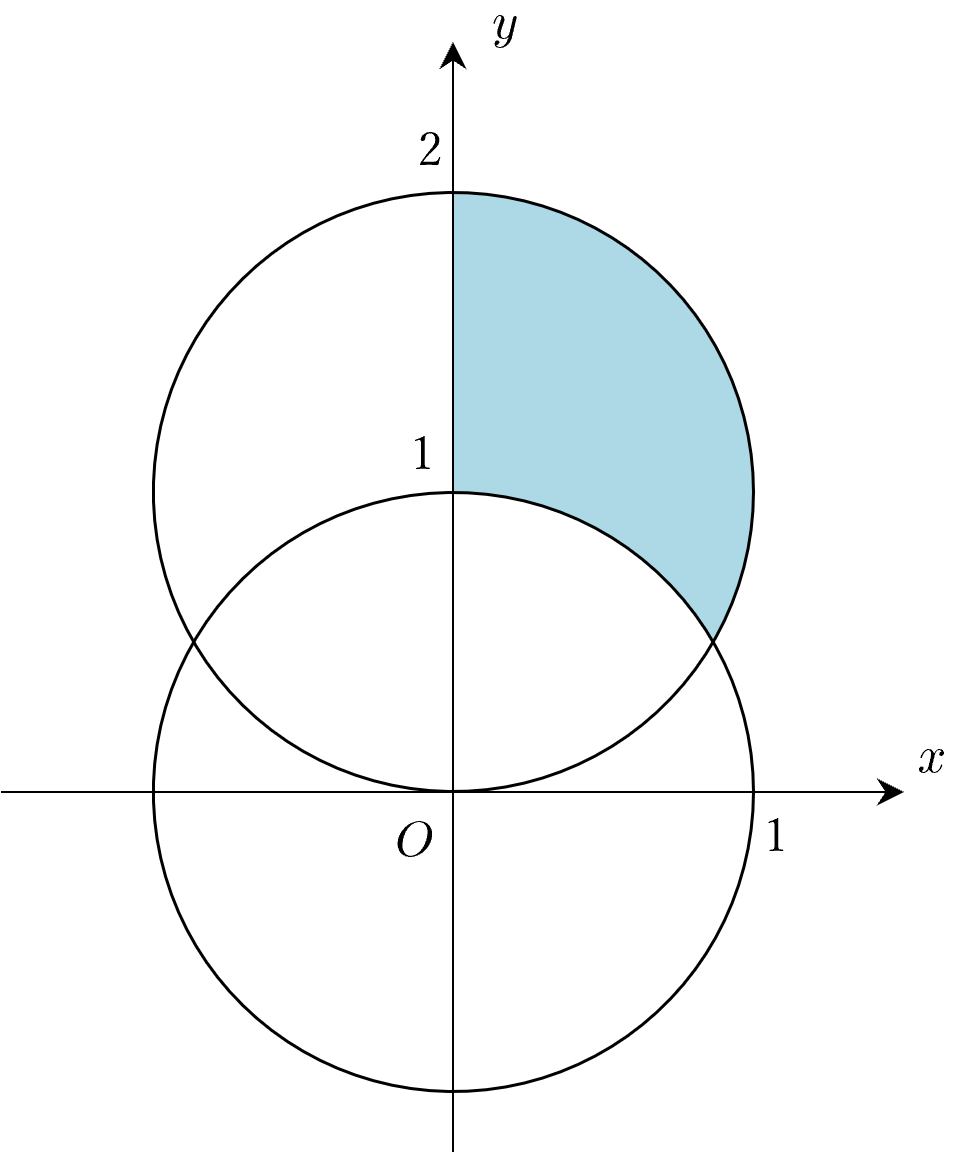
\includegraphics[width=.5\linewidth]{./src/fig/Basic/B_2023_autumn_D.png}
    \end{figure}

    \item
    与えられた積分について極座標変換\dm{x = r\cos\grt,\,y=r\sin\grt}を考えると、
    領域\dm{D}は
    \begin{align}
      D &= \Dset{(r,\grt)\relmiddle r\geq 0, 0\leq\grt\leq\frac{\pi}{2}, 1\leq r^2 \leq 2r\sin\grt}\\
        &= \Dset{(r,\grt)\relmiddle r\geq 0, 0\leq\grt\leq\frac{\pi}{2}, 1\leq r \leq 2\sin\grt}\\
        &= \Dset{(r,\grt)\relmiddle 0\leq\grt\leq\frac{\pi}{2}, 1\leq r \leq 2\sin\grt}\\
        &= \Dset{(r,\grt)\relmiddle \frac{\pi}{6}\leq\grt\leq\frac{\pi}{2}, 1\leq r \leq 2\sin\grt}\quad(\because 1\leq 2\sin\grt)
    \end{align}
    である。\dm{dxdy = r\,drd\grt}も考えて、
    \begin{align}
      I
      &= \int_{\pi/6}^{\pi/2}\int_{1}^{2\sin\grt} r^2\cos\grt \,drd\grt  \\
      &= \int_{\pi/6}^{\pi/2}d\grt \left[ \frac{r^3}{3}\cos\grt \right]_{1}^{2\sin\grt} \\
      &= \int_{\pi/6}^{\pi/2}\left( \frac{8}{3}\sin^3\grt\cos\grt - \frac{1}{3}\cos\grt \right) \,d\grt \\
      &= \frac{1}{3}\int_{1/2}^{1}(8t^3-1) \,dt \\
      &= \frac{1}{3}\left[ 2t^4 - t \right]_{1/2}^{1} \\
      &= \frac{11}{24}
    \end{align}
  \end{enumerate}
\end{ans*}
\begin{other*}
  領域\dm{D}は
  \begin{align}
    D
    &= \left\{(x,y)\relmiddle x\geq 0, y\geq 0, 1\leq x^2 + y^2\leq 2y\right\} \\
    \begin{split}
      &= \left\{(x,y)\relmiddle 0\leq x\leq \frac{\sqrt{3}}{2}, \sqrt{1-x^2}\leq y\leq \sqrt{1-x^2}+1 \right\} \\
      &\hspace*{50pt} \vee \left\{(x,y)\relmiddle \frac{\sqrt{3}}{2}\leq x\leq 1, -\sqrt{1-x^2}+1\leq y\leq \sqrt{1-x^2}+1 \right\}
    \end{split}
  \end{align}
  とも表せるので、重積分\dm{I}は
  \begin{align}
    I
    &= \int_{0}^{\sqrt{3}/2}\int_{\sqrt{1-x^2}}^{\sqrt{1-x^2}+1} x\,dydx
       + \int_{\sqrt{3}}^{1}\int_{-\sqrt{1-x^2}+1}^{\sqrt{1-x^2}+1}x\,dydx \\
    &= \int_{0}^{\sqrt{3}/2} x \,dx + \int_{\sqrt{3}/2}^{1}2x\sqrt{1-x^2}\,dx \\
    &= \left[\frac{1}{2}x^2\right]_{0}^{\sqrt{3}/2} + \int_{3/4}^{1}\sqrt{1-t}\,dt \quad(t=x^2) \\
    &= \frac{1}{2}\cdot\frac{3}{4} + \left[-\frac{2}{3}(1-t)^{3/2}\right]_{3/4}^{1} \\
    &= \frac{11}{24}
  \end{align}
\end{other*}



\subsection{線形代数}
\prob{%
  ベクトル\dm{\ba}および\dm{\bb}に関する以下の問いに答えよ。
  \begin{align}
    \ba =
    \pmat{
      \:\: 1 \:\:\:\\ 2 \\ 1
    }
    ,\quad
    \bb =
    \pmat{
    \:\:  -4 \:\:\:\\ 11 \\ 6
    }
  \end{align}
  \begin{enumerate}[label=(\arabic*)]
    \item ベクトル\dm{\bb}を、\dm{\ba}を通る直線へ射影せよ。
    \item \dm{\ba}を通る直線への射影行列\dm{\bm{P}}を求めよ。
  \end{enumerate}
}
\begin{ans*}
  ${}$
  \begin{enumerate}[label=(\arabic*)]
    \item $\ba$と$\bb$のなす角を$\grt$とし、
    ベクトル$\bb$ の$\ba$ への射影ベクトルを$\bp$とする。
    \begin{align}
      \bm{p}=\proj_{\ba} \bb
      &= \frac{\|\bp\|}{\|\ba\|}\ba \\
      &= \frac{\|\bb\|\cos\grt}{\|\ba\|}\ba \\
      &= \frac{\|\bb\|\ip{\ba,\bb}}{\|\ba\|^2\|\bb\|}\ba \\
      &= \frac{\ip{\ba,\bb}}{\|\ba\|^2}\:\ba \\
      &=
      4
      \Bmat{
      \:\:  1 \:\:\:\\ 2 \\ 1 \\
      }
    \end{align}
    \item
    射影行列は任意のベクトル$\bx\in\bbR^3$を$\ba$への射影に変換する線形写像である。
    すなわち(1)より$\ba$への射影ベクトル$\proj_{\ba}\bx$が$\bP\bx$と等しいとき
    \begin{gather}
      \bP\bx = \proj_{\ba}\bx = \frac{\ip{\ba,\bx}}{\|\ba\|^2} \ba = \frac{\ba^\top \bx}{\ba^{\top}\ba}\ba
    \end{gather}
    ここで、$\ba^{\top}\bx \in \bbR$であるので、
    \begin{align}
      \frac{\ba^\top \bx}{\ba^{\top}\ba}\ba
      &= \frac{\ba (\ba^{\top} \bx)}{\ba^{\top}\ba} \\
      &= \frac{\ba\ba^{\top}}{\ba^{\top}\ba}\bx
    \end{align}
    である。これが$\bP\bx$と等しいので
    \begin{gather}
      \bP = \frac{\ba\ba^{\top}}{\ba^{\top}\ba}
    \end{gather}
    として射影行列$\bP$を得る。
    \begin{align}
      \bm{P}
      = \frac{1}{6}
      \begin{bmatrix}
        1 & 2 & 1 \\ 2 & 4 & 2 \\ 1 & 2 & 1
      \end{bmatrix}
    \end{align}
  \end{enumerate}
\end{ans*}

\prob{%
  \dm{\bA = \bL\bU}とする下三角行列\dm{\bL}と上三角行列\dm{\bU}を求めよ。
  ただし、下三角行列\dm{\bL}の対角成分は1とする。
  \begin{align}
    \bA =
    \pmat{
      a & a & a \\
      a & b & b \\
      a & b & c
    }
  \end{align}
}
\begin{ans*}
  行列\dm{\bL,\bU}の未知の\dm{i}行\dm{j}列の要素を
  \dm{l_{ij},u_{ij}}と表すとき、
  \dm{\bL\bU}分解は
  \begin{align}
    \bA
    &=
    \bL\bU \\
    &=
    \bmat{
      1 & 0 & 0 \\
      l_{21} & 1 & 0 \\
      l_{31} & l_{32} & 1 \\
    }
    \bmat{
      u_{11} & u_{12} & u_{13} \\
      0 & u_{22} & u_{23} \\
      0 & 0 & u_{33} \\
    } \\
    &=
    \bmat{
      u_{11} & u_{12} & u_{13} \\
      l_{21}u_{11} & l_{21}u_{12}+u_{22} & l_{21}u_{13}+u_{23} \\
      l_{31}u_{11} & l_{31}u_{12}+l_{32}u_{22} & l_{31}u_{13}+l_{32}u_{23}+u_{33} \\
    }
  \end{align}
  とできるので、
  \begin{gather}
    \bL =
    \bmat{
      1& 0& 0 \\
      1& 1& 0 \\
      1& 1& 1 \\
    } \\
    \bU =
    \bmat{
      a& a& a \\
      0& b-a& b-a \\
      0& 0& c-b \\
    }
  \end{gather}
\end{ans*}

\prob{%
  行列\dm{\bB}に関する以下の問いに答えよ。
  \begin{align}\bB =
    \pmat{
      {\displaystyle \frac{5}{6}} & {\displaystyle \frac{1}{3}} \\
      \\
      {\displaystyle \frac{1}{6}} & {\displaystyle \frac{2}{3}} \\
    }
  \end{align}
  \begin{enumerate}[label=(\arabic*)]
    \item \dm{\bB}の固有値をすべて求めよ。
    \item \dm{\bB^2}の固有値をすべて求めよ。
    \item \dm{\bB^{\infty}}を求めよ。
  \end{enumerate}
}
\begin{ans*}
  ${}$
  \begin{enumerate}[label=(\arabic*)]
    \item \bB の固有方程式\dm{\det(\bB-\grl\bE)=0}より
    \begin{align}
      \det(\bB-\grl\bE)
      &=
      \biggl(\grl-\frac{5}{6}\biggr)\biggl(\grl-\frac{2}{3}\biggr)-\frac{1}{18} \\
      &= \frac{1}{2}(\grl - 1)(2\grl - 1) = 0 \\
      &\therefore \grl = \frac{1}{2}, 1
    \end{align}
    \item
    \dm{\bB^2}は
    \begin{gather}
      \bB^2 =
      \bmat{
        {\disp \frac{3}{4}} & {\disp \frac{1}{2}} \\
        \\
        {\disp \frac{1}{4}} & {\disp \frac{1}{2}} \\
      }
    \end{gather}
    であるので、\dm{\bB^2} の固有方程式\dm{\det(\bB^2-\grl\bE)=0}より
    \begin{align}
      \det(\bB^2-\grl\bE)
      &=
      \biggl(\grl-\frac{3}{4}\biggr)\biggl(\grl-\frac{1}{2}\biggr)-\frac{1}{8} \\
      &= \frac{1}{4}(\grl - 1)(4\grl - 1) = 0 \\
      &\therefore \grl = \frac{1}{4}, 1
    \end{align}

    \item
    \bB は対角化行列\bP を用いて
    \begin{gather}
      \bP^{-1}\bB\bP =
      \bmat{
        {\disp \frac{1}{2}} & 0 \\
        \\
        0 & {1} \\
      }
    \end{gather}
    と対角化される。このとき対角化行列\bP について

    \begin{enumerate}[label=(\roman*)]
      \item \dm{\grl = \frac{1}{2}}のとき
      \begin{gather}
        (\bB -\grl\bE)\bu = \bm{0} \\
        \bu = \Bmat{ x \\ y } \\
        \Rightarrow
        \bmat{
          {\disp\frac{1}{3}} & {\disp\frac{1}{3}} \\&\\ {\disp\frac{1}{6}} & {\disp\frac{1}{6}}
        }
        \Bmat{
          x \\ y
        }
        =\bm{0}
      \end{gather}
      であるので、固有ベクトルは
      \begin{gather}
        \bu_{1} =
        \Bmat{
          1 \\ -1
        }
      \end{gather}
      \item \dm{\grl = 1}のとき
      \begin{gather}
        (\bB -\grl\bE)\bu = \bm{0} \\
        \bu = \Bmat{ x \\ y } \\
        \Rightarrow
        \bmat{
          {\disp -\frac{1}{6}} & {\disp\frac{1}{3}} \\&\\ {\disp\frac{1}{6}} & {\disp -\frac{1}{3}}
        }
        \Bmat{
          x \\ y
        }
        =\bm{0}
      \end{gather}
      であるので、固有ベクトルは
      \begin{gather}
        \bu_{2} =
        \Bmat{
          2 \\ 1
        }
      \end{gather}
    \end{enumerate}

    (i)、(ii)より、対角化行列\bP は
    \begin{gather}
      \bP =
      \bmat{
        1 & 2 \\-1 & 1
      } \\
      \bP^{-1} = \frac{1}{3}
      \bmat{
        1 & -2 \\1 & 1
      }
    \end{gather}
    ゆえに
    \begin{align}
      (\bP^{-1}\bB\bP)^{\infty}
      &= \bP^{-1}\bB^{\infty}\bP\\
      &=
      \bmat{
        \biggl({\disp \frac{1}{2}}\biggr)^{\infty} & 0 \\ & \\ 0 & 1
      } =
      \bmat{
        0 & 0 \\ 0 & 1
      }
    \end{align}
    左から$\bP$、右から$\bP^{-1}$をかけて
    \begin{align}
      \bB^{\infty}
      &=
      \bmat{
        1 & 2 \\
        -1 & 1 \\
      }
      \bmat{
        0 & 0 \\
        0 & 1 \\
      }
      \cdot\frac{1}{3}
      \bmat{
        1 & -2 \\
        1 & 1 \\
      }\\
      &= \frac{1}{3}
      \bmat{
        2 & 2 \\
        1 & 1 \\
      }
    \end{align}
  \end{enumerate}
\end{ans*}
